\begin{figure*}[!t]
        \centering{
                \begin{tabular}{cccc}
                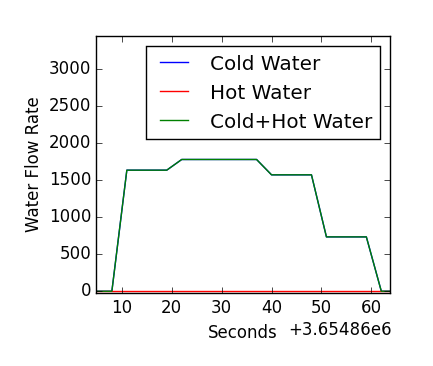
\includegraphics[width=1.6in]{multidisaggfig/UpToilet.png}&
                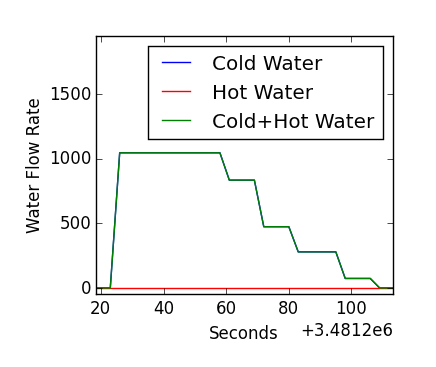
\includegraphics[width=1.6in]{multidisaggfig/DownToilet.png}&
                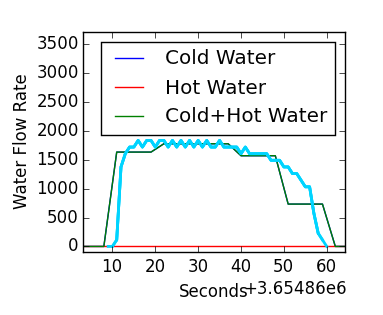
\includegraphics[width=1.6in]{multidisaggfig/UpToiletFitted.png}&
                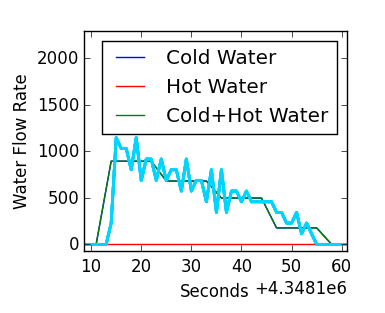
\includegraphics[width=1.6in]{multidisaggfig/DownToiletFitted.png}
                \tabularnewline
                (a) & (b) & (c) & (d) \tabularnewline
                \end{tabular}
                }
        \caption{
        (a) and (b) denote two complete usage cycles of down toilet and up toilet in dataset study10. X-axis is seconds, 
Y-axis is water flow rate in 10000*liter/minute. (c) and (d) Disaggregation of two toilets by dynamic time warping subsequence search. 
The cyan denote the original up toilet and down toilet patterns which are discovered by feature extraction. }
        \label{fig_UpToiletDownToilet}
\end{figure*}